% Technical report — Proyecto Nota 3: Big Data with Python and PySpark (English version)
% Build from this folder:  pdflatex report.tex  (twice, for the table of contents)
\documentclass[11pt,a4paper]{article}

\usepackage[utf8]{inputenc}
\usepackage[T1]{fontenc}
\usepackage[english]{babel}
\usepackage{lmodern}
\usepackage[margin=2.5cm]{geometry}
\usepackage{graphicx}
\usepackage{booktabs}
\usepackage{tabularx}
\usepackage{xcolor}
\usepackage{listings}
\usepackage{caption}
\usepackage{float}
\usepackage[hidelinks]{hyperref}

\graphicspath{{../../graficos/}}

\definecolor{codebg}{HTML}{F6F6F4}
\definecolor{codecomment}{HTML}{52514E}
\definecolor{pending}{HTML}{B3261E}

\lstset{
  language=Python,
  basicstyle=\ttfamily\small,
  backgroundcolor=\color{codebg},
  commentstyle=\color{codecomment}\itshape,
  keywordstyle=\bfseries,
  frame=single,
  rulecolor=\color{codebg},
  breaklines=true,
  columns=fullflexible,
  keepspaces=true,
  showstringspaces=false,
  captionpos=b
}
\renewcommand{\lstlistingname}{Listing}

% Visible marker for what is still missing before submission.
\newcommand{\pending}[1]{\textcolor{pending}{\textbf{[PENDING: #1]}}}

\title{Processing 67 million Amazon reviews:\\
pandas versus Apache Spark (PySpark)\\[0.4em]
\large Proyecto Nota 3 --- Big Data with Python and PySpark}
\author{Cristhian Eduardo Osorio Restrepo \and Daniel Stiven Pérez Córdoba \and Maria Camargo\\[0.3em]
\small Professor: Ing. Luis Fernando Castro Rojas, Mg, PhD.}
\date{November 2026}

\begin{document}
\maketitle
\tableofcontents
\newpage

% ---------------------------------------------------------------------------
\section{Introduction and problem statement}

\subsection{Domain and problem}

E-commerce produces millions of product reviews every day. A store or seller that wants to
understand them needs to answer simple questions over very large volumes: when activity
peaks, which stores receive the most reviews and how good their ratings are, and which
records are incomplete.

This project answers five business questions about the Amazon \emph{Home and Kitchen}
reviews:

\begin{enumerate}
  \item How does the number of reviews behave over time (year, month and weekday)?
  \item Which stores concentrate the largest volume of reviews?
  \item What is the mean rating and its spread in each group?
  \item Which records are incomplete or inconsistent?
  \item Which reviews have, and which lack, their product in the catalog?
\end{enumerate}

Answering them requires the operations the assignment asks for: reading, cleaning, derived
columns, a join with the product catalog, group-by aggregations and writing the results to
Parquet.

\subsection{Data}

The project uses the \emph{Amazon Reviews 2023} dataset from the McAuley Lab at the
University of California San Diego~\cite{hou2024}, published on Hugging Face. Files are
downloaded through direct URLs, without running any code from the source repository.

\begin{table}[H]
\centering
\caption{Files used from the \emph{Home and Kitchen} category. Sizes checked from the HTTP
headers on 17 November 2026.}
\label{tab:data}
\begin{tabularx}{\textwidth}{lXrr}
\toprule
File & Content & Size & Records \\
\midrule
\texttt{0core/rating\_only} (CSV) & User--product interactions: user, product, rating and date & 3.86 GB & 66,623,880 \\
\texttt{meta\_Home\_and\_Kitchen} (JSONL) & Product catalog: category, store, price & 11.8 GB & 3,735,584 \\
\texttt{review\_categories} (JSONL) & Full reviews, with title and text & 31.4 GB & --- \\
\bottomrule
\end{tabularx}
\end{table}

The measurements in Section~\ref{sec:evidence} were first taken with the interactions CSV,
joined with the catalog. The full-review file, which carries the text, is used for the
volume test: it was converted once to Parquet with an explicit schema (67\,409\,944
reviews, 9.72 GB, 8 columns) and sampled at 1, 10, 50 and 100\,\%, always joined with the
same full catalog.

\subsection{Why is this a Big Data problem?}

\begin{itemize}
  \item \textbf{Volume.} The full-review file is 31.4 GB, twice the RAM of the test machine
  (15.3 GB). The interactions alone are 66.6 million rows.
  \item \textbf{Variety.} Tabular data (CSV) is combined with semi-structured data (one JSON
  object per line) that includes free text.
  \item \textbf{Memory, not disk.} A compressed or columnar file takes far less space on disk
  than once loaded into memory. In the measurements, joining the interactions with the
  catalog produces a pandas \emph{DataFrame} of about 12 GB, at the limit of the machine's
  15.3 GB.
\end{itemize}

The project's hypothesis is that, on the same machine, pandas stops being viable when the
volume exceeds the available memory, while Spark completes the work because it processes
data partition by partition.

% ---------------------------------------------------------------------------
\section{Theoretical background}

\subsection{Big Data}

Data is called Big Data when its volume, arrival speed or variety exceeds what a traditional
tool can process in reasonable time and with reasonable resources. The usual answer is to
\emph{scale out}: split the data into parts and process them in parallel, on several cores
or several machines, instead of relying on one bigger machine.

\subsection{Apache Spark architecture}

Apache Spark is an open-source distributed processing engine~\cite{zaharia2016,chambers2018}. Its main
parts are:

\begin{description}
  \item[Driver.] The process that runs the user's program. It builds the execution plan,
  splits it into tasks and schedules them. It must not receive all the data: calling
  \texttt{collect()} on a large dataset runs the driver out of memory.
  \item[Executors.] The processes that run the tasks on the data. In the local mode used
  here (\texttt{local[*]}), driver and executors live in the same Java virtual machine, with
  one execution thread per core.
  \item[Partitions.] Data is split into blocks called partitions. Each task processes one
  partition, so the whole dataset never has to be in memory at once. If a partition does not
  fit, Spark writes intermediate data to disk (\emph{spill}) instead of failing.
  \item[Transformations and actions.] Transformations (\texttt{filter},
  \texttt{withColumn}, \texttt{join}, \texttt{groupBy}) describe a new dataset without
  computing it. Actions (\texttt{count}, \texttt{write}, \texttt{collect}) request a result
  and trigger execution.
  \item[Lazy evaluation.] Because transformations are not executed immediately, Spark knows
  the whole plan before running it. That lets it, for instance, read only the columns in use
  or filter before joining.
  \item[DAG.] The plan is a directed acyclic graph of operations. Spark cuts it into
  \emph{stages} wherever data must be redistributed across partitions (a \emph{shuffle}),
  such as a \texttt{groupBy} or a \texttt{join}. The shuffle is the most expensive operation,
  because it moves data between tasks and writes it to disk.
\end{description}

On top of this core, the DataFrame API and Spark SQL~\cite{armbrust2015} add the
\emph{Catalyst} optimizer, which rewrites the logical plan before execution, and since
Spark~3 \emph{adaptive query execution} (AQE), which adjusts the plan with real statistics,
for example by merging small partitions~\cite{sparkdocs}.

\subsection{Optimization techniques used}

\begin{description}
  \item[Parquet.] A columnar, compressed format~\cite{parquet}. Since each column is stored
  separately, a query reads only the columns it needs (\emph{column pruning}).
  \item[Broadcast join.] When one of the two tables is small, it is copied in full to every
  executor and the large table is joined where it already is, with no shuffle.
  \item[Caching.] Keeps an intermediate result in memory when it is reused several times, so
  it is not recomputed. It only pays off when recomputing costs more than storing.
  \item[Shuffle partitions.] By default Spark creates 200 partitions per shuffle; on a single
  machine that means many tiny tasks. Sizing them to the number of cores lowers the
  scheduling cost.
\end{description}

\subsection{Limitations of pandas}

pandas~\cite{mckinney2010} is the reference library for tabular data analysis in Python,
but it was designed for a single node and for data that fits in memory:

\begin{itemize}
  \item \textbf{Everything in memory.} It loads the whole dataset into RAM before operating.
  If it does not fit, the process ends with \texttt{MemoryError} or the operating system
  kills it.
  \item \textbf{Eager execution.} Each operation runs immediately and creates complete
  intermediate results; a \texttt{merge} may need both the original and the joined table at
  the same time.
  \item \textbf{One core.} Most operations use a single core, even on a multi-core machine.
\end{itemize}

pandas has its own mitigations: reading only some columns, using smaller data types or
processing the file in parts (\emph{chunks}). The pandas documentation itself recommends
them~\cite{pandasscale}. Section~\ref{sec:evidence} shows how far they go.

% ---------------------------------------------------------------------------
\section{Environment and configuration on Windows}

\subsection{Machines}

All measurements ran on a single Windows machine, with the same configuration for pandas and
Spark. The Linux machine was used only to develop and test the code.

\begin{table}[H]
\centering
\caption{Machines and software versions.}
\label{tab:environment}
\begin{tabularx}{\textwidth}{lXX}
\toprule
 & Measurement machine & Development machine \\
\midrule
Operating system & Windows 11 Home & Debian 13 (Linux) \\
Processor & AMD Ryzen 5 7520U, 4 cores and 8 threads & 16 threads \\
RAM & 15.3 GB & 15.3 GB \\
Free disk & 300 GB & 13 GB \\
Python & 3.13.17 & 3.13.5 \\
Java & Microsoft OpenJDK 17.0.21 & Temurin 17.0.18 \\
\midrule
PySpark & \multicolumn{2}{l}{4.3.0 (bundles Spark)} \\
pandas / pyarrow / psutil & \multicolumn{2}{l}{3.1.1 / 26.0.1 / 7.2.2} \\
\bottomrule
\end{tabularx}
\end{table}

\subsection{Installation}

The full installation guide is in the repository's \texttt{README.md}. In short:

\begin{enumerate}
  \item Python 3.13 through \texttt{winget}, always invoked with the \texttt{py -3.13}
  launcher.
  \item JDK 17 through \texttt{winget}; the installer sets \texttt{JAVA\_HOME}.
  \item \texttt{winutils.exe} and \texttt{hadoop.dll} from Hadoop 3.3.6 with the
  \texttt{scripts/setup\_winutils.ps1} script, which checks their SHA-256 and sets
  \texttt{HADOOP\_HOME}.
  \item A virtual environment from \texttt{requirements.txt}, which pins exact versions.
\end{enumerate}

\texttt{SPARK\_HOME} is not needed: the \texttt{pyspark} package from PyPI bundles the full
Spark distribution and locates it by itself. This is stated explicitly because the
assignment mentions that variable.

\subsection{Problems found and how they were solved}

\begin{table}[H]
\centering
\small
\caption{Environment problems recorded in the project log.}
\label{tab:problems}
\begin{tabularx}{\textwidth}{XX}
\toprule
Problem & Solution \\
\midrule
Only Python 3.14 was installed, outside the range PySpark 4.3.0 supports (3.11--3.13), and the \texttt{python} command opened the Microsoft Store. &
Install Python 3.13 with \texttt{winget} and always use \texttt{py -3.13}. \\
There was no Java and no \texttt{JAVA\_HOME}. &
Install Microsoft OpenJDK 17 with \texttt{winget}, which asks for elevation and sets the variable. \\
Writing Parquet failed: first because \texttt{HADOOP\_HOME} was missing, then with \texttt{UnsatisfiedLinkError} because \texttt{hadoop.dll} was missing. &
A script downloads \texttt{winutils.exe} and \texttt{hadoop.dll}, checks their SHA-256 and sets \texttt{HADOOP\_HOME} and \texttt{PATH} without administrator rights. \\
The script itself did not start on PowerShell 5.1: a syntax error in \texttt{"\$name: ..."} and broken accents when reading UTF-8 without a BOM. &
Use \texttt{"\$\{name\}: ..."}, save with a BOM and add an automated test that checks the script syntax. \\
PySpark 4.3.0 warns that it does not fully support pandas 3. &
No effect on the tests; pandas 3.1.1 is kept so that the measurements already taken stay valid. \\
Downloads of large files could not be resumed: a network drop meant starting over. &
Resumable download: the partial \texttt{.part} file is kept and the transfer continues with an HTTP \texttt{Range} request. \\
\bottomrule
\end{tabularx}
\end{table}

% ---------------------------------------------------------------------------
\section{Source code analysis}

\subsection{Organization}

The repository separates what is delivered from what is measured:

\begin{itemize}
  \item \texttt{pandas\_version/analysis.py} and \texttt{spark\_version/analysis.py} contain
  the same six operations, one function per operation, with the same names.
  \item \texttt{spark\_version/optimized.py} reuses those Spark functions and only changes
  \emph{how} they run.
  \item \texttt{benchmark/} imports those same functions to measure them. What is measured is
  exactly what is delivered.
  \item \texttt{tests/} checks that pandas and Spark produce the same results on the same
  data.
\end{itemize}

The shared rules are written down in a contract
(\texttt{docs/CONTRATO\_ANALISIS\_amazon\_hk.md}): same columns, same cleaning rules, same
weekday numbering and a $10^{-4}$ tolerance on means and standard deviations.

\subsection{Reading}

Spark reads with an \textbf{explicit schema}. Without it, Spark would have to scan the file
once just to infer each column's type, which over tens of gigabytes is a full extra pass.

\begin{lstlisting}[caption={Explicit catalog schema in Spark.}]
META_SCHEMA = StructType([
    StructField("parent_asin", StringType(), True),
    StructField("store", StringType(), True),
    StructField("price", DoubleType(), True),
    # ... other catalog columns
])
spark.read.schema(META_SCHEMA).json(str(meta_path)) \
    .filter(F.col("parent_asin").isNotNull()) \
    .dropDuplicates(["parent_asin"])
\end{lstlisting}

Nothing is loaded yet at this point: reading is a transformation. pandas, instead, loads the
whole file into memory as soon as \texttt{read\_parquet} is called.

\subsection{Cleaning}

Both versions apply the same three rules: drop rows with nulls in the key columns, keep
ratings between 1 and 5, and keep positive timestamps.

\begin{lstlisting}[caption={Cleaning in pandas (top) and Spark (bottom).}]
cleaned = reviews.dropna(subset=["user_id", "parent_asin", "rating", "timestamp"])
cleaned = cleaned[(cleaned["rating"] >= 1) & (cleaned["rating"] <= 5)
                  & (cleaned["timestamp"] > 0)]

reviews.dropna(subset=["user_id", "parent_asin", "rating", "timestamp"]) \
    .filter((F.col("rating") >= 1) & (F.col("rating") <= 5) & (F.col("timestamp") > 0))
\end{lstlisting}

The syntax is almost the same, but the effect is not: pandas creates a filtered copy of the
whole table right away, while Spark only adds a step to the plan. That step runs later,
partition by partition, and the optimizer places it as close to the read as possible.

\subsection{Derived columns}

Both versions turn the timestamp (milliseconds since 1970, in UTC) into year, month, weekday
and hour. The delicate detail is the \textbf{weekday}: pandas numbers it from 0 (Monday) to
6 (Sunday) and Spark from 1 (Sunday) to 7 (Saturday). pandas is aligned with Spark:

\begin{lstlisting}[caption={Converting the pandas weekday to Spark's numbering.}]
derived["review_dow"] = ((review_ts.dt.dayofweek + 1) % 7) + 1
# Monday: ((0 + 1) % 7) + 1 = 2   -> same as Spark
# Sunday: ((6 + 1) % 7) + 1 = 1   -> same as Spark
\end{lstlisting}

Without this conversion the temporal table would differ between engines even though both
were correctly written. An automated test checks all seven days.

\subsection{Join with the catalog}

It is a \textbf{left} join on \texttt{parent\_asin}: every review is kept, and those whose
product is missing from the catalog get an empty store. They are not dropped, because they
answer question~5.

\begin{lstlisting}[caption={Join in pandas, baseline Spark and optimized Spark.}]
reviews.merge(catalog, on="parent_asin", how="left")          # pandas
reviews.join(catalog, "parent_asin", "left")                  # baseline Spark
reviews.join(F.broadcast(catalog), "parent_asin", "left")     # optimized Spark
\end{lstlisting}

In pandas, \texttt{merge} builds the full joined table in memory; it is the most
memory-hungry step. In baseline Spark, the join requires a shuffle of both tables by
\texttt{parent\_asin}. In the optimized version the catalog is reduced to two columns and
broadcast to every executor, so the reviews are joined where they are, without moving them.

\subsection{Aggregations}

\begin{lstlisting}[caption={Store aggregate in pandas (top) and Spark (bottom).}]
reviews.groupby("store", dropna=False).agg(
    reviews=("parent_asin", "size"),
    products=("parent_asin", "nunique"),
    avg_rating=("rating", "mean"),
    stddev_rating=("rating", "std"))

reviews.groupBy("store").agg(
    F.count("*").alias("reviews"),
    F.countDistinct("parent_asin").alias("products"),
    F.round(F.avg("rating"), 4).alias("avg_rating"),
    F.round(F.stddev("rating"), 4).alias("stddev_rating"))
\end{lstlisting}

Two decisions make them agree:

\begin{itemize}
  \item \texttt{dropna=False} in pandas keeps the group of reviews with no store. Spark keeps
  the null group by default; pandas would drop it without that option.
  \item The standard deviation is the \textbf{sample} one in both: pandas \texttt{std} and
  Spark \texttt{stddev} divide by $n-1$.
\end{itemize}

In Spark, a \texttt{groupBy} runs in two phases: each partition aggregates its own rows, the
partial results are shuffled, and then they are combined. Only partial results move, not the
original rows.

\subsection{Writing}

pandas writes one Parquet file per table. Spark writes a \emph{folder} with one file per
partition, because each task writes its own part in parallel. Since the aggregated tables
are small, the optimized version applies \texttt{coalesce(1)} to leave one file per table.

Writing is also the \textbf{action} that triggers all the previous computation. That is why,
in the per-operation measurements, Spark's write time includes the reading, cleaning, join
and aggregations that until then were only planned.

\subsection{Optimized version and its relation to the DAG}

\texttt{spark\_version/optimized.py} reuses the functions above and changes the execution in
five points, plus an optional cache. Each one can be switched on or off from the command
line to measure its effect.

\begin{table}[H]
\centering
\small
\caption{Optimizations of the Spark version and the concept each applies.}
\label{tab:optimizations}
\begin{tabularx}{\textwidth}{lXl}
\toprule
Optimization & What changes & Concept \\
\midrule
Read 4 columns & Parquet does not read the other columns from disk & Columnar format \\
Temporal table without join & The temporal table uses no catalog column; it is computed without the join & DAG: one shuffle less \\
Broadcast join & The catalog, reduced to 2 columns, is copied to every executor & Broadcast join \\
Shuffle partitions & 2 per core instead of 200 & Partitions \\
One file per table & \texttt{coalesce(1)} before writing & Partitions \\
Cache (off) & Would keep the cleaned reviews for both aggregations & Caching \\
\bottomrule
\end{tabularx}
\end{table}

The effect is visible in the physical plan Spark builds before running (\texttt{explain}).
For the store table, the join appears as \texttt{BroadcastHashJoin} and the read asks only
for the needed columns:

\begin{lstlisting}[language={},caption={Physical plan of the store table (optimized version).}]
AdaptiveSparkPlan
+- HashAggregate                          <- combines the partial results
   +- Exchange                            <- shuffle (new stage)
      +- HashAggregate                    <- aggregates inside each partition
         +- ...
            +- BroadcastHashJoin LeftOuter BuildRight
               :- Filter <- Scan parquet  (user_id, parent_asin, rating, timestamp)
               +- BroadcastExchange
                  +- Filter <- Scan parquet  (parent_asin, store)
\end{lstlisting}

The plan of the temporal table contains no \emph{join} at all: only read, filter, projection
and aggregation.

In a test with 20 million synthetic reviews on the Linux machine, the optimized version
produced tables identical to the baseline and took 25.7 to 26.1 seconds, against 27.1 to
27.7 for the baseline. With the cache on it was slower (28.8 to 29.2 seconds): re-reading
four Parquet columns cost less than storing 20 million rows in memory. That is why the cache
is off by default. On the Windows machine, with the full 100\,\% sample (67.4 million reviews
with text), the optimized version took \textbf{123.4 seconds} end to end and produced the same
tables as the baseline: 67\,409\,944 rows, 375\,506 stores and 1\,985 time groups.

% ---------------------------------------------------------------------------
\section{Evidence that pandas is not viable}
\label{sec:evidence}

All measurements were taken on the Windows machine (8 logical cores, 15.3 GB of RAM), with
the full-review data that includes the text. Every figure in this section comes from
\path{docs/evidencia/measurements_raw_text.csv}. Each run starts in a fresh process; a
memory guard kills the whole process tree, JVM included, when system RAM reaches about
98\,\%, records the kill as the result, and waits for the system to recover before the next
run. At the kill it records the \emph{private} (committed) memory, because Windows trims the
resident set of a process under pressure and the resident value understates the real demand.

\subsection{Naive attempt}

Reading the 31.4 GB review file directly with \texttt{pd.read\_json} committed
\textbf{30\,305 MB of private memory in 20.1 seconds}, twice the RAM of the machine, before
the guard stopped it at 98\,\% of system RAM.

\subsection{Sample ladder}

\begin{table}[H]
\centering
\caption{Outcome per sample and engine (raw-text route). pandas: mean of 3 repetitions;
Spark: 3 repetitions at 1 and 10\,\%, 1 at 50 and 100\,\%.}
\label{tab:ladder}
\small
\begin{tabularx}{\textwidth}{rrXX}
\toprule
Sample & Reviews & pandas & Spark \\
\midrule
1\,\%   & 673\,379    & finishes, peak 1\,335 MB & finishes, peak 3\,842 MB \\
10\,\%  & 6\,742\,408  & finishes, peak 4\,694 MB & finishes, peak 4\,157 MB \\
50\,\%  & 33\,706\,117 & \textbf{killed} 3/3 at 97--98\,\% RAM (12\,966--13\,131 MB private) & finishes, peak 5\,281 MB \\
100\,\% & 67\,409\,944 & \textbf{killed} 3/3 at 98--99\,\% RAM (13\,894--14\,580 MB private) & finishes, peak 5\,897 MB \\
\bottomrule
\end{tabularx}
\end{table}

pandas needs the whole table in memory at once, so its memory grows with the data: it does
not finish even half of the reviews. Spark processes the data partition by partition and
spills to disk, so its peak stays under 6 GB from 1\,\% to 100\,\%
(Figure~\ref{fig:memory}).

\begin{figure}[H]
\centering
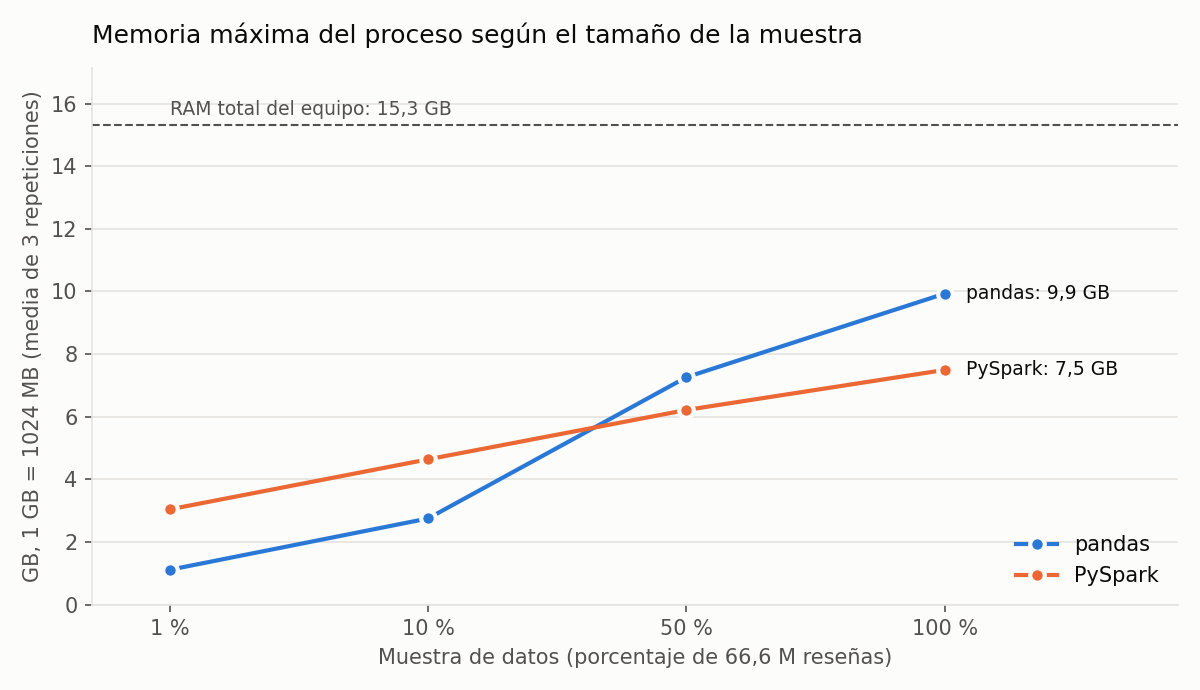
\includegraphics[width=0.9\textwidth]{memoria_pico.png}
\caption{Peak memory per sample. An X marks a pandas run killed by the guard, at the private
memory it had committed; the dashed line is the machine's RAM.}
\label{fig:memory}
\end{figure}

\subsection{System screenshots}

\begin{figure}[H]
\centering
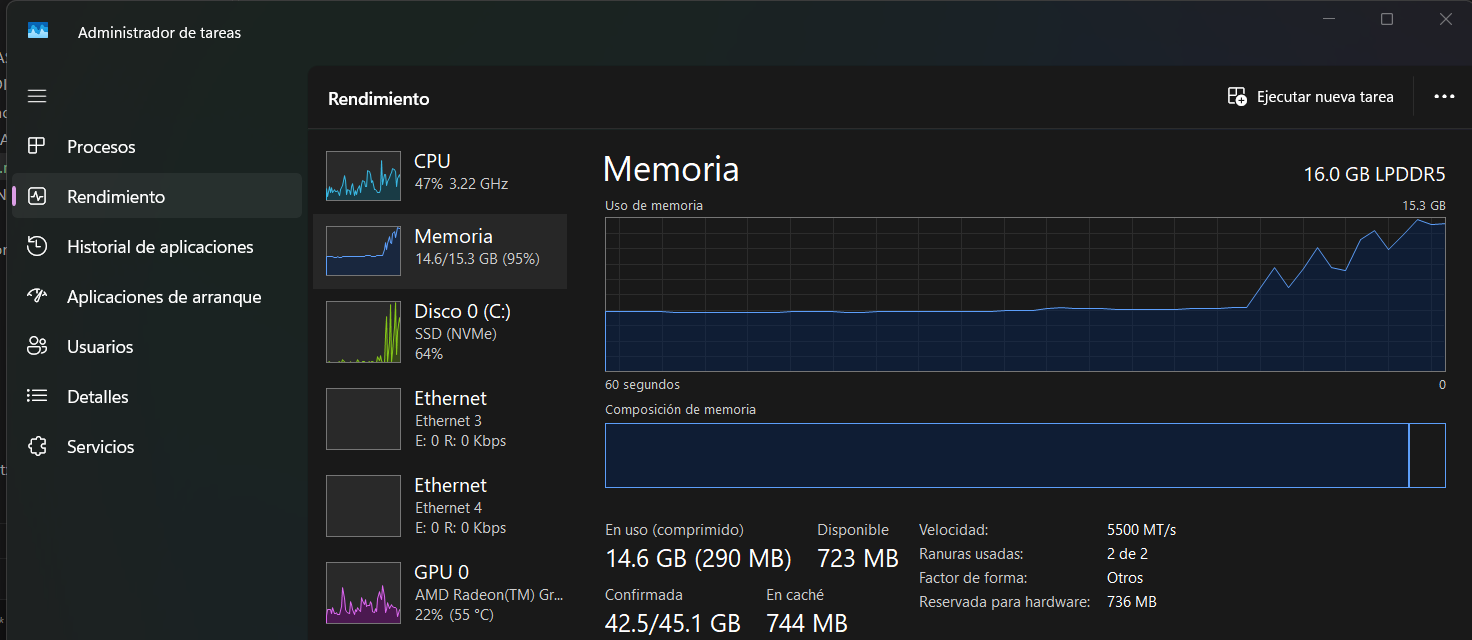
\includegraphics[width=0.85\textwidth]{../../evidencia/capturas/pandas_fallo_memoria.png}
\caption{Task Manager while pandas processes the data: memory in use climbs to 95\,\% (14.6 of
15.3 GB) with 42.5 GB committed; the guard kills such runs at 97--99\,\%.}
\label{fig:shot-pandas}
\end{figure}

\begin{figure}[H]
\centering
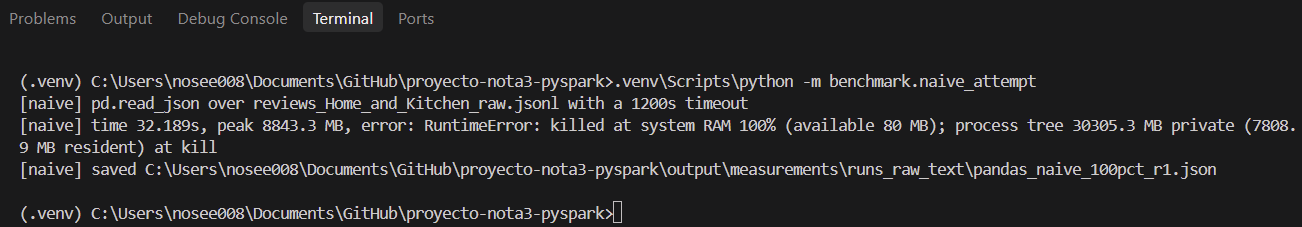
\includegraphics[width=0.85\textwidth]{../../evidencia/capturas/pandas_error_terminal.png}
\caption{The kill recorded in the terminal: system RAM at 98\,\% and 30\,305 MB of private
memory committed.}
\label{fig:shot-error}
\end{figure}

\begin{figure}[H]
\centering
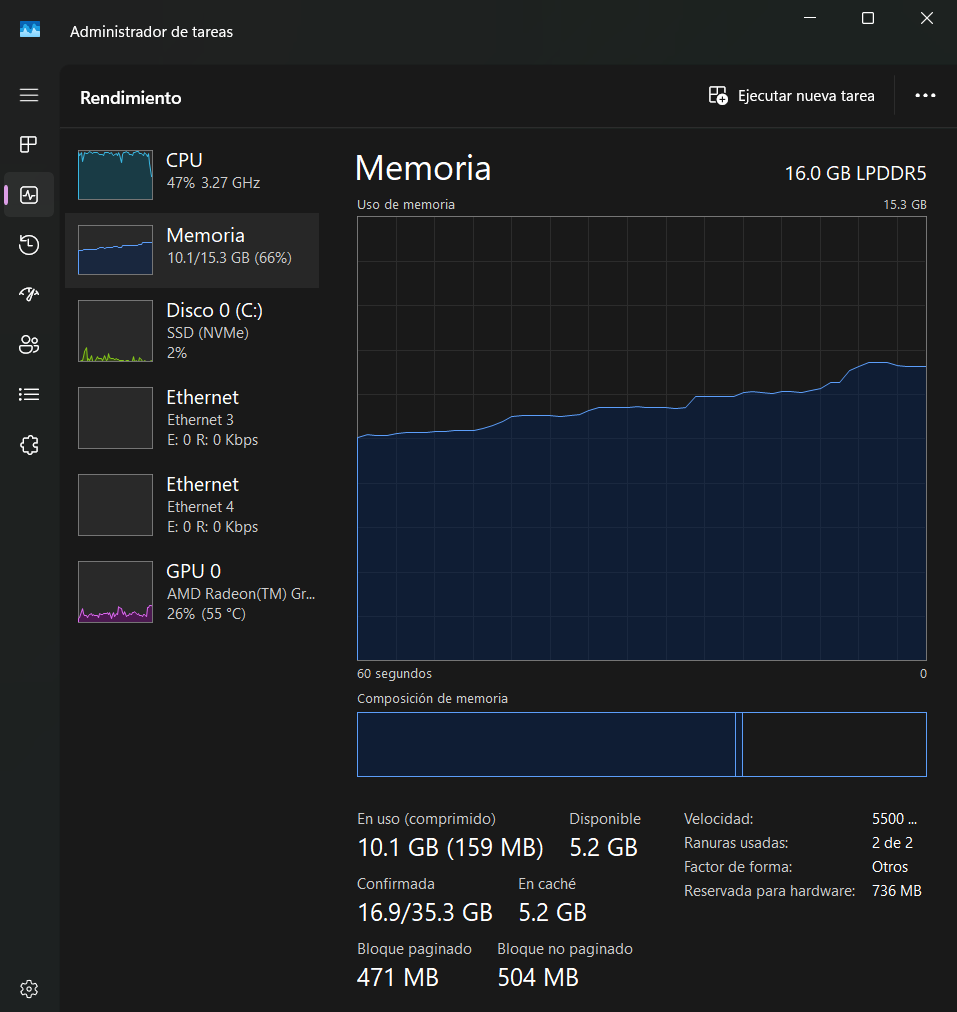
\includegraphics[width=0.85\textwidth]{../../evidencia/capturas/spark_100_memoria.png}
\caption{Task Manager while Spark finishes the 100\,\% sample: memory in use for the whole
system (other programs included) stays stable at about 10 GB, below the 15.3 GB of RAM. The
Spark process tree alone peaked at 5\,897 MB (Table~\ref{tab:ladder}).}
\label{fig:shot-spark}
\end{figure}

\begin{figure}[H]
\centering
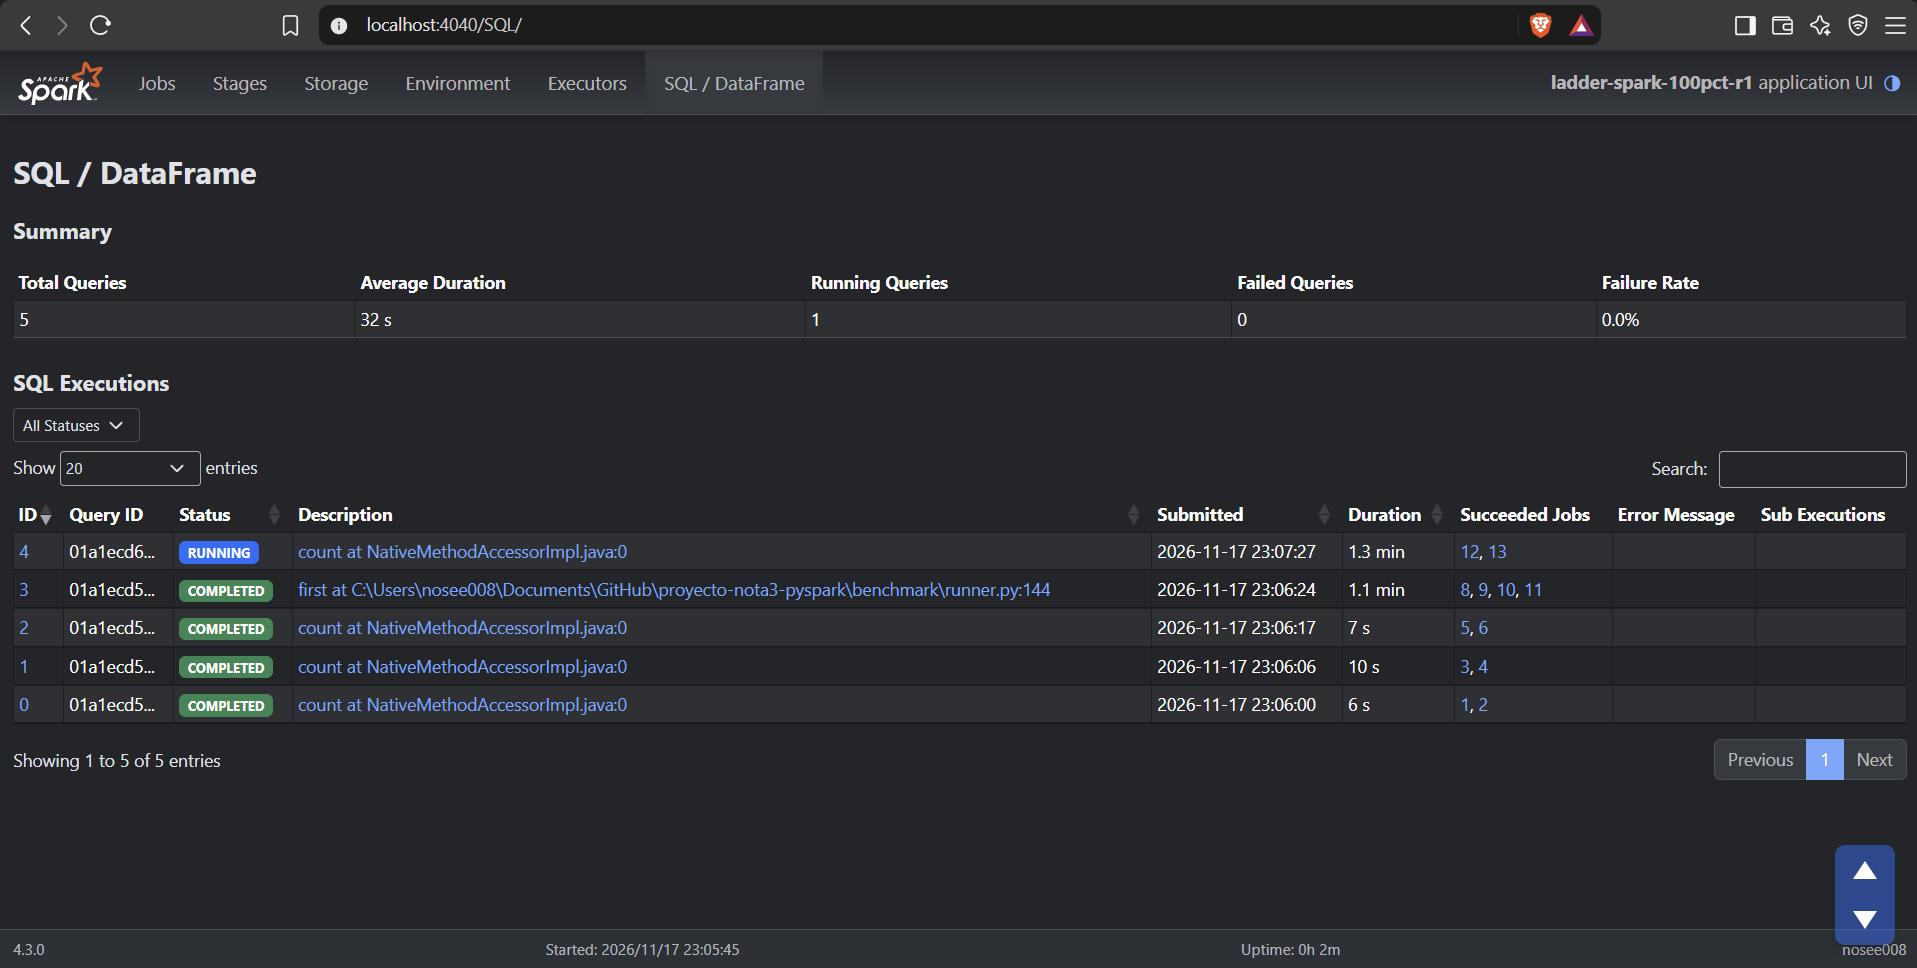
\includegraphics[width=0.85\textwidth]{../../evidencia/capturas/spark_ui_dag.png}
\caption{Spark UI (\texttt{localhost:4040}) during the 100\,\% run, showing the job plan.}
\label{fig:shot-ui}
\end{figure}

\subsection{pandas mitigations}

Before declaring pandas not viable, its own techniques were tried. All three were implemented
(\path{pandas_version/mitigated.py}) and measured with the same instrument
(\path{docs/evidencia/mitigaciones.csv}).

\begin{table}[H]
\centering
\caption{pandas mitigations on the 100\,\% sample (67.4 million reviews with text).}
\label{tab:mitigations}
\begin{tabular}{llrr}
\toprule
Technique & Outcome & Time (s) & Peak (MB) \\
\midrule
Only the needed columns & killed at 98\,\% RAM & --- & 10\,663 \\
Smaller dtypes & killed at 97\,\% RAM & --- & 10\,223 \\
Chunks + partial aggregation & finishes & 3\,460 & 427$^{\ast}$ \\
\bottomrule
\end{tabular}
\smallskip

\footnotesize{$^{\ast}$Sets of ASINs per store that must stay alive to compute
\texttt{products}. Spark builds both tables in 214.6 s (one pass).}
\end{table}

The first two techniques finish up to 10\,\% and die afterwards: the review text is a contract
column (needed for \texttt{avg\_text\_length}), it cannot be dropped or narrowed, and its bytes
are what fill the memory. Reading in chunks is the only technique that finishes 100\,\%, but at
a price: 57.7 minutes against 3.6 for one Spark pass (about 16 times slower), keeping
3\,734\,414 ASINs alive in per-store sets just to compute \texttt{products}, and with no way to
express global operations (sorting 67 million rows, percentiles, windows) without reading
everything again. None of them brings pandas to a practical 100\,\% run: either it does not
finish, or it finishes sixteen times slower with part of the logic rewritten by hand
\cite{pandasscale}.

% ---------------------------------------------------------------------------
\section{Comparative analysis: pandas versus Spark}

\subsection{How time is measured}

The benchmark times each Spark operation with an action (\texttt{count}) and caches nothing.
Because Spark is lazy, each action re-executes the plan from the read: the time of the
``join'' step already includes reading, cleaning and deriving. Adding all the steps would
count the same work several times (52.7 s instead of 12.2 s at 1\,\%). One full pass of the
Spark pipeline is therefore the \texttt{write\_parquet} operation alone, which builds both
tables from scratch. pandas is eager, so the sum of its steps is one pass. This is an
estimate: when the write runs, the operating system already caches the input file.
As a check, the optimized version run end to end on the 100\,\% sample took 123.4 seconds,
below that one-pass estimate of the baseline.

\begin{table}[H]
\centering
\caption{Time of one full pass (seconds, mean of the finished runs).}
\label{tab:time}
\begin{tabular}{rrrr}
\toprule
Sample & pandas & Spark & Spark $\div$ pandas \\
\midrule
1\,\%   & 4.7  & 12.2  & 2.6 \\
10\,\%  & 27.8 & 32.3  & 1.2 \\
50\,\%  & ---  & 161.3 & --- \\
100\,\% & ---  & 214.6 & --- \\
\bottomrule
\end{tabular}
\end{table}

\begin{figure}[H]
\centering
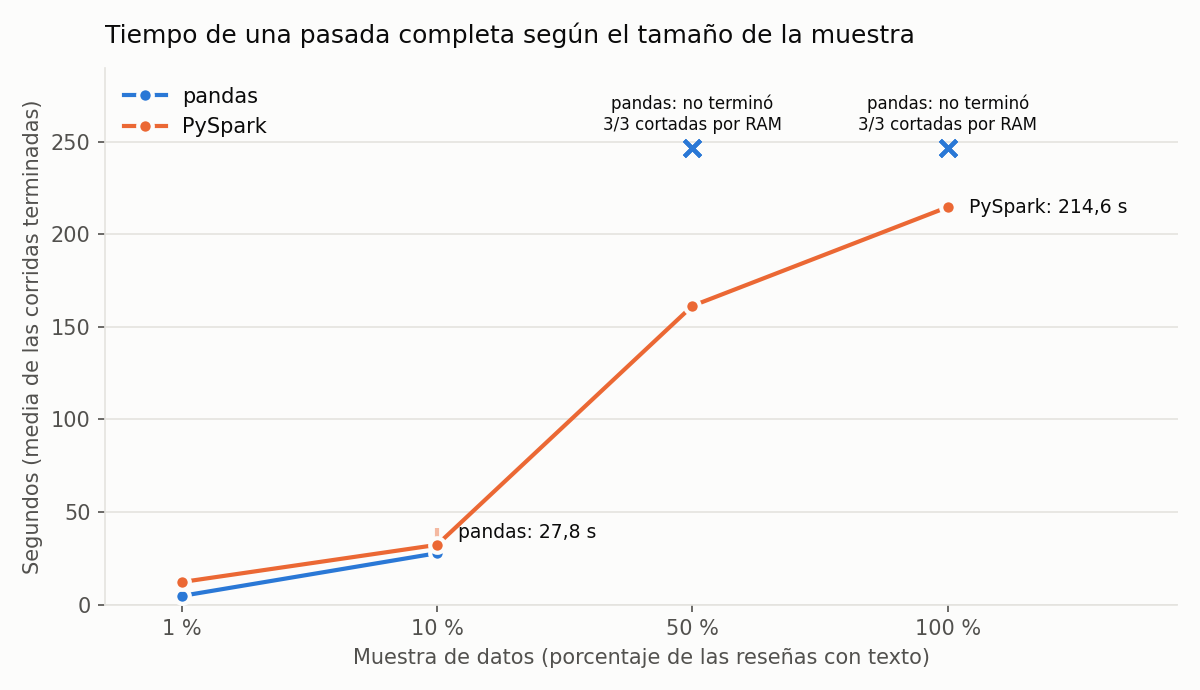
\includegraphics[width=0.9\textwidth]{tiempo_total.png}
\caption{Time of one full pass per sample. pandas did not finish at 50 and 100\,\%.}
\label{fig:time}
\end{figure}

\subsection{Discussion}

\begin{itemize}
  \item \textbf{Small data: pandas wins.} At 1\,\% pandas is 2.6 times faster: Spark pays a
  fixed cost (starting the JVM, planning, scheduling tasks) that small data does not pay back.
  \item \textbf{The gap closes as data grows.} At 10\,\% Spark takes only 1.2 times as long.
  \item \textbf{Large data: only Spark finishes.} At 50 and 100\,\% pandas runs out of memory,
  while Spark processes all 67.4 million reviews in about 3.6 minutes with less than 6 GB.
  \item \textbf{Same results.} Where both finish (1 and 10\,\%) the tables are identical:
  9 of 9 compared pairs, the same groups and the same top store, and 0 reviews without catalog.
  \item \textbf{Optimizations have a break-even point.} The optimized version is 1.74 times
  faster at 100\,\% (123.4 s against 214.6) but slower at 10\,\% (39.3 s against 32.3): the
  broadcast and the column pruning do not pay for themselves with a few million rows.
\end{itemize}

Per operation (Figure~\ref{fig:ops}), pandas is faster at every in-memory step. The Spark bars
are cumulative because of the re-execution explained above, which is itself a direct effect of
lazy evaluation without caching.

\begin{figure}[H]
\centering
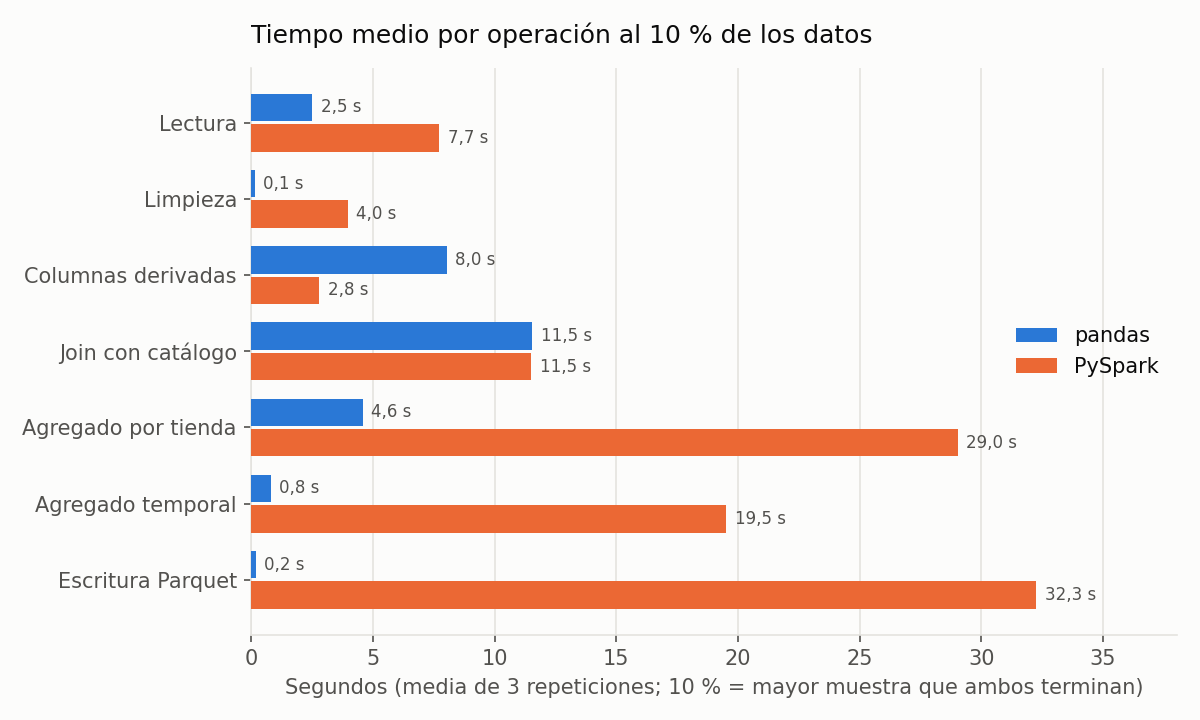
\includegraphics[width=0.9\textwidth]{tiempo_por_operacion_10.png}
\caption{Mean time per operation at 10\,\%, the largest sample both engines finish.}
\label{fig:ops}
\end{figure}

% ---------------------------------------------------------------------------
\section{Conclusions}

\begin{enumerate}
  \item The hypothesis holds: on a 15.3 GB machine pandas cannot process the reviews with
  their text from 50\,\% of the data upward, and the naive read commits 30.3 GB in 20 seconds.
  Spark finishes 100\,\% (67.4 million reviews) with a peak below 6 GB.
  \item Spark is not faster on small data: at 1\,\% pandas is 2.6 times faster. Spark is the
  right tool when the data no longer fits in memory, not by default.
  \item Lazy evaluation matters when measuring: without caching, each action recomputes the
  whole plan, and summing per-step times overstates Spark's cost 2.7 to 4.3 times.
  \item The optimized version (column pruning, broadcast join, no join for the temporal table,
  shuffle partitions sized to the machine) gives the same tables as the baseline: 123.4 s
  against 214.6 for one pass (1.74 times faster) at 100\,\%, although at small scale its cost
  does not pay off.
  \item The pandas mitigations are not enough: column selection and compact dtypes die at 50
  and 100\,\% because the text is part of the analysis, and chunks finish but 16 times slower
  and with part of the logic rewritten by hand. pandas is not viable \emph{even when mitigated}
  for this volume on this machine.
\end{enumerate}

% ---------------------------------------------------------------------------
\begin{thebibliography}{9}

\bibitem{hou2024}
Y.~Hou, J.~Li, X.~Fu, Z.~He, A.~Yan, X.~Chen, and J.~McAuley, ``Bridging language and items
for retrieval and recommendation: Benchmarking LLMs as semantic encoders,'' \emph{arXiv
preprint arXiv:2403.03952v2}, 2024.

\bibitem{zaharia2016}
M.~Zaharia \emph{et al.}, ``Apache Spark: A unified engine for big data processing,''
\emph{Communications of the ACM}, vol.~59, no.~11, pp.~56--65, 2016.

\bibitem{armbrust2015}
M.~Armbrust \emph{et al.}, ``Spark SQL: Relational data processing in Spark,'' in
\emph{Proc. ACM \mbox{SIGMOD} International Conference on Management of Data}, 2015,
pp.~1383--1394.

\bibitem{mckinney2010}
W.~McKinney, ``Data structures for statistical computing in Python,'' in \emph{Proc. 9th
Python in Science Conference (SciPy)}, 2010, pp.~56--61.

\bibitem{chambers2018}
B.~Chambers and M.~Zaharia, \emph{Spark: The Definitive Guide: Big Data Processing Made
Simple}. Sebastopol, CA, USA:
O'Reilly Media, 2018.

\bibitem{sparkdocs}
The Apache Software Foundation, ``Spark SQL and DataFrames,'' Apache Spark 4.3.0
documentation. [Online]. Available:
\url{https://spark.apache.org/docs/4.3.0/sql-programming-guide.html}. Accessed: Nov. 17,
2026.

\bibitem{parquet}
The Apache Software Foundation, ``Documentation,'' Apache Parquet. [Online]. Available:
\url{https://parquet.apache.org/docs/}. Accessed: Nov. 17, 2026.

\bibitem{pandasscale}
pandas development team, ``Scaling to large datasets,'' pandas 3.1.1 documentation.
[Online]. Available: \url{https://pandas.pydata.org/docs/user_guide/scale.html}.
Accessed: Nov. 17, 2026.

\end{thebibliography}

\end{document}
